% 三角形基本：顶点 A B C, 边 a b c (a=BC, b=CA, c=AB)
\documentclass[tikz,border=4pt]{standalone}
\usepackage{ctex}
\usepackage{amsmath}
\usetikzlibrary{calc}
\begin{document}
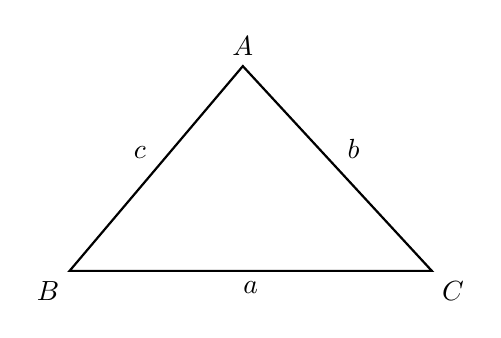
\begin{tikzpicture}[scale=1.0, thick]
  \coordinate (A) at (0, 2.6);
  \coordinate (B) at (-2.2, 0);
  \coordinate (C) at (2.4, 0);
  \draw (A) -- (B) -- (C) -- cycle;
  \node[above]      at (A) {$A$};
  \node[below left] at (B) {$B$};
  \node[below right]at (C) {$C$};
  \node[below]      at ($(B)!0.5!(C)$) {$a$};
  \node[above right] at ($(C)!0.5!(A)$) {$b$};
  \node[above left]  at ($(A)!0.5!(B)$) {$c$};
\end{tikzpicture}
\end{document}
